\documentclass[russian]{beamer}

\usepackage{cmap} % для кодировки шрифтов в pdf
\usepackage[T2A]{fontenc}
\usepackage[utf8]{inputenc}
\usepackage[russian]{babel}
\usepackage{minted} % code highlighting

\usepackage{graphicx} % для вставки картинок
\graphicspath{ {img/} }

%\usetheme{Warsaw}
%\usecolortheme{beaver}

\title[Интерполяция]{Алгоритмы интерполяции функций.\newline Создание библиотеки на языке Clojure.}
\author{Белоглазов Никита}
\date{2013}
\institute{Белорусский Государственный Университет}

\begin{document}

\maketitle
\begin{frame}[fragile]
  \frametitle{Clojure}
  \definecolor{bg}{rgb}{0.95,0.95,0.95}
  \begin{minted}[bgcolor=bg,gobble=4,frame=single]{clojure}
    (defn derivative [f x]
      (let [h 0.00001]
        (/ (- (f (+ x h))
              (f x))
           h)))

    (defn f1 [x] x)       ; f1(x) = x
    (defn f2 [x] (* x x)) ; f2(x) = x * x

    (derivative f1 0) ; f1'(0) = 1
    (derivative f2 0) ; f2'(0) = 0.00001
    (derivative f2 4) ; f2'(4) = 8.00001
  \end{minted}
\end{frame}

\begin{frame}
  \frametitle{Incanter}

  \emph{Incanter} - математический R-подобный пакет для алгебраических и статистических расчётов на языке Clojure.

  \begin{itemize}

  \item Функции для построения графиков и визуализации данных.

  \item Математические функции.

  \item Статистические функции.

  \item Функции для работы с матрицами и линейной алгеброй.

  \item Функции обработки данных.

  \item \emph{Функции построения интерполирующих функций.}
  \end{itemize}
\end{frame}

\begin{frame}
  \frametitle{Интерполяция}
  \begin{center}
    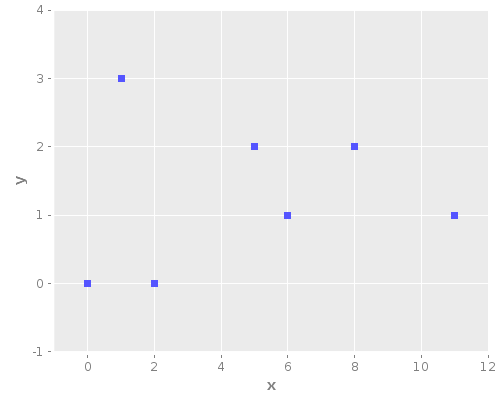
\includegraphics[width=.4\textwidth,height=.4\textheight,keepaspectratio]{points}
    \\
    ?
  \end{center}
  \begin{columns}[c]
    \begin{column}{.35\textwidth}
      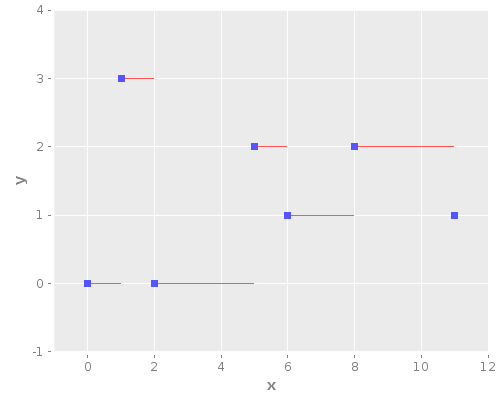
\includegraphics[width=\textwidth,height=\textheight,keepaspectratio]{interrupted}
    \end{column}
    \begin{column}{.35\textwidth}
      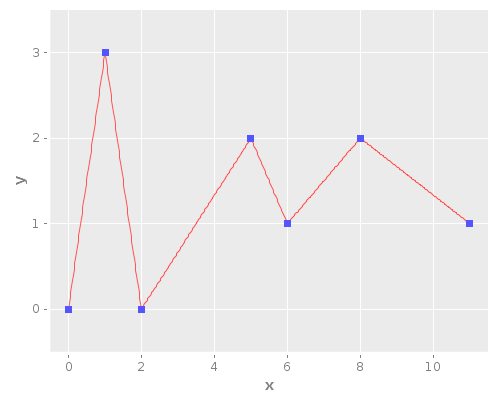
\includegraphics[width=\textwidth,height=\textheight,keepaspectratio]{linear_interpolation_1_var_small}
    \end{column}
    \begin{column}{.35\textwidth}
      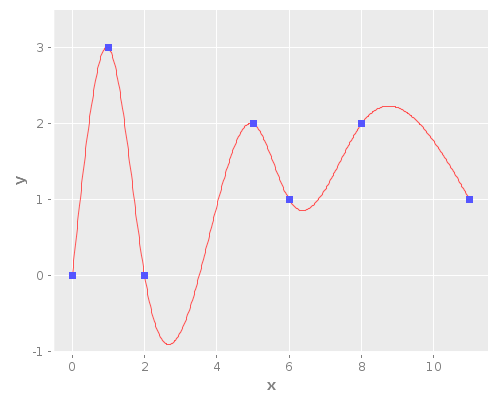
\includegraphics[width=\textwidth,height=\textheight,keepaspectratio]{cubic_interpolation_1_var_small}
    \end{column}
  \end{columns}
\end{frame}

\end{document}

%%% Local Variables:
%%% mode: latex
%%% TeX-master: t
%%% End:
